\section{Implementation}
\label{sec:implementation}

This section outlines the technical implementation of the blockchain-based LEM simulation
and presents parts of the developed source code. Therefore, we give a brief introduction to the applied 
software technologies and present the individual components and their containing attributes and functions.
Finally, we present the simulation process that we divided into \textit{Initial Setup} and \textit{Main Simulation Loop}. 

\subsection{Applied Technologies}
\label{sec:applied_technologies}
In this subsection we give a brief introduction 
to the applied software technologies and libraries.

\paragraph{Python}
An interpreted, object-oriented, high-level programming language with dynamic semantics. 
Additionally, it is simple and comes with an easy to learn syntax \footnote{https://www.python.org/}.
The programming language of choice, which is used to develop the 
respective components that communicate via the blockchain.

\paragraph{Web3.py}
A Python library for interacting with an Ethereum blockchain \footnote{https://github.com/ethereum/web3.py}. 
It enables the developed Python components to communicate via the blockchain.

\paragraph{Ganache}
A personal blockchain for Ethereum development \footnote{https://github.com/trufflesuite/ganache-cli}.
It simulates a full client behavior and makes developing Ethereum applications faster, easier and safer.
Ganache is provided on the one hand as a software tool with a graphical user interface (GUI) and on the other hand as command-line tool (CLI). In the develop LEM simulation the command line version of Ganache is used. 

\paragraph{Solidity}
A statically typed, contract-oriented, high-level programming language for implementing smart contracts on the Ethereum
blockchain \footnote{https://github.com/ethereum/solidity}.
It is used to implement the smart contract dealer. 

\clearpage
%--------------------------------------
\subsection{Components}
\label{sec:components_of_simulation}
We present the three main components \textit{Agent},\textit{Smart Contract Dealer} and \textit{Off-chain Dealer} 
in this subsection and introduce their attributes and functions. 

\subsubsection{Agent}
\label{sec:agent_class}
The agents are implemented by a Python class and the naming is oriented on the proposed BTM.
As stated in section \ref{sec:concept_of_lem}, the agents represent the respective households in the BLEMS. 
First, the class attributes are presented and the associated source code is shown
in the following Listing \ref{lst:agent_class_attributes}.

\begin{lstlisting}[label=lst:agent_class_attributes, caption=Overview of the agent class attributes, language=Python]
    class Agent(object):

    def __init__(self, agent_number, account_address, web3, dealer_contract):
        self._name = 'AGENT{}'.format(agent_number)
        self._account_address = account_address
        self._web3 = web3
        self._dealer_contract = dealer_contract
        self._optimization_problem = None
        self._bundle_set = None
        self._bid = None
        self._mkt_prices = None
        self._trade = None
        self._objective = None
        self._wealth = None
        self._accept_trade = None
\end{lstlisting}

The variables \verb|agent_number|, \verb|account_address|, \verb|web3| and \verb|dealer_contract| are initialized when the class is instantiated.
The variable \verb|agent_number| is used to identify the different agents.
Due to its uniqueness, the \verb|account_address| could be also used as an identifier, 
but it would be cumbersome due to the cryptic hexadecimal representation of the blockchain account addresses.
Therefore a more comprehensible name for each agent is established.
Furthermore, each agent is assigned an Ethereum blockchain account defined by the variable \verb|account_address|. It is required to submit and 
receive transactions via the blockchain.
The Python library for interacting with an Ethereum blockchain is represented by the variable \verb|web3|.
Moreover, the \verb|dealer_contract| constitues an object of the dealer's smart contract that knows all of its implemented functions.
Hence, this variable is needed to call the functions of the smart contract out of this Python class.
All other presented class attributes in the Listing are set during the simulation process.\\

Next, some of the essential functions of the class are introduced and described in detail.

The agents require a function for receiving their optimization problems, which 
implementation is presented in Listing \ref{lst:lp_setter}.

\begin{lstlisting}[label=lst:lp_setter, caption=Setter of optimization problem, language=Python]
    @optimization_problem.setter
    def optimization_problem(self, value):
        self._optimization_problem = value
        self._objective = self._optimization_problem.solve().fun
        self._wealth = self.balance + abs(self._objective)
\end{lstlisting}

After setting the optimization problem, the class attributes \verb|objective| and \verb|wealth| are determined.
In this case, the attribute \verb|wealth| is defined exactly as in the BTM. 
The \verb|balance| constitues the cash endowment $e_{j}$ and \verb|objective| the optimal value of the agents
problem depending on the current amount of the shared resources $z_{j}(c_{j})$.
However, \verb|balance| is not a class attribute, but a class function that uses 
\verb|web3| and \verb|account_address| to retrieve the current
balance of the account from the blockchain.

In addition, the implementation of the function for solving the BDP and hence determining 
the improving bundle set and the associated bid is introduced in the Listing \ref{lst:determine_bundle}.

\begin{lstlisting}[label=lst:determine_bundle, caption=Determining of bundle attributes, language=Python]
    def determine_bundle_attributes(self):
        result = solve_bundle_determination(self._optimization_problem, self._mkt_prices)
        self._bundle_set = result.x
        self._bid = self._objective - result.fun
\end{lstlisting}

First, the BDP is solved in a separate function in subject to the optimization problem and the current market prices.
The associated source code of the function can be found in the appendix \ref{appendix:additional_agent}.

The \verb|bundle_set| constitutes the improving bundle set and is assigned from the results of the BDP.
Further, the \verb|bid| is initialized. We stated that the BTM implemented nonstrategic bidding and pricing,
wherefore an agent always submits a limit price equal to the valuation of the bundle, such that $l(w) = v(w)$.
The value of \verb|bid| is assigned by the difference of the \verb|objective| $z_{j}(c_{j})$ and the 
objective of the optimization problem with the additional resources of the \verb|bundle_set| $z_{j}(c_{j}+w)$, 
which reflects the definition of the bundles true value $v(w) = z_{j}(c_{j}) - z_{j}(c_{j}+w)$.

Next, Listing \ref{lst:set_order} presents the implementation of the function for 
submitting orders to the dealer's smart contract.
Currently, smart contracts in Ethereum do not fully 
support fixed point numbers. It is possible to declare them, but they cannot be assigned to or from \shortcite{solidity_fixed_point}.
This poses a problem because the values in the BTM often contain fixed point numbers. Therefore, 
we developed a workaround that shifts the decimal places to the right and truncates
the remainder when values sent to the dealer's smart contract so that integer values are generated.
When obtaining values from the dealer's smart contract we shift the decimal places to the left to restore 
the original fixed point values. 
Due to this, the \verb|bundle_set| and \verb|bid| are prepared for 
sending to the dealer's smart contract.

\begin{lstlisting}[float=htbp, label=lst:set_order, caption=Submitting of order, language=Python]
    def set_order(self):
        bundle_set = utils.prepare_for_sending(self._bundle_set)
        bid = utils.prepare_for_sending(self._bid)
        
        if(bid > 0):
            prepayment = utils.from_ether_to_wei(self._bid)
        else:
            prepayment = 0

        self._dealer_contract.contract.functions.setOrder(bundle_set, bid, prepayment).transact({'from': self._account_address, 'value': prepayment})
\end{lstlisting}

Additionally, it is identified if the \verb|bid| represents a buy or a sell order by examining if the value 
of \verb|bid| is greater than zero. In case of a buy order, the agents have to pay in advance, to which 
the variable \verb|prepayment| is assigned in the amount of \verb|bid|.
We implemented this procedure to prevent the strategic placing of orders and to ensure 
that the financial resources are available.
In case of a sell order, no payment in advance is required and the \verb|prepayment| is set to zero.
Moreover, Wei is a subdivision of the cryptographic currency of Ethereum and presents the base unit within smart contracts.
As 1 Ether is defined as $10^{-18}$ Wei, we decided to specify all monetary values on the side 
of the agents and the off-chain dealer in Ether for better clarity.
Therefore, the \verb|bid| is converted from Ether to Wei before assigning to the \verb|prepayment|.
Finally, the \verb|dealer_contract| is used to call the function of the dealer's smart contract which is
responsible for setting the orders.

Moving calculations off the blockchain comes along with the drawback that source code is not
transparent to all agents anymore. 
That comes to bear in the opacity of the trade calculation of the dealer. 
To adress this issue we implemented a trade verification procedure based on 
strong duality theory, which implementation is outlined in Listing \ref{lst:verify_trade}.
The verification procedure applies the Strong Duality Theorem to verify the validity of the off-chain dealer's calculations.
That means, if the primal MMP has an optimal solution $x^{*}$, then 
the dual also has an optimal solution $y^{*}$, such that $c^{T}x^{*} = b^{T}y^{*}$.
Due to this, it is possible to verify if the solution of the dealer is optimal, without solving the corresponding MMP. 
The agents calculate whether strong duality holds and decide on the basis of the result whether they accept the trade or not.
Because of the limitations of floating point arithmetic \footnote{https://docs.python.org/2/tutorial/floatingpoint.html}, 
we round off the values of the MMP and the dual problem to make sure that correct trades 
are not rejected based on limited machine accuracy.
Finally, the class variable \verb|accept_trade| is assigned according to the result of the trade verification 
procedure.

\begin{lstlisting}[float=htbp, label=lst:verify_trade, caption=Verification of trades, language=Python]
    def verify_strong_duality(self):
        mmp_values, mmp_duals, mmp_target_coefs, mmp_bounds = self.get_mmp_attributes()
        primal_solution = (-np.sum(mmp_values * mmp_target_coefs))
        dual_solution = np.sum(mmp_duals * mmp_bounds)
        primal_solution = math.floor(primal_solution * 10) / 10
        dual_solution = math.floor(dual_solution * 10) / 10

        if primal_solution == dual_solution:
            self._accept_trade = True
        else:
            self._accept_trade = False
\end{lstlisting}


Likewise, the class contains a function for notifing the dealer's smart contract if the respective trade is accepted or not,
as shown in the Listing \ref{lst:accept_trade}.

\begin{lstlisting}[float=htbp, label=lst:accept_trade, caption=Notification of trade acceptance, language=Python]
    def accept_trade(self):
        if(self._accept_trade):
            trade = self._dealer_contract.contract.functions.acceptTrade(self._accept_trade).call({'from': self._account_address})
            self._trade = utils.prepare_for_storing(trade)

        self._dealer_contract.contract.functions.acceptTrade(self._accept_trade).transact({'from': self._account_address})

\end{lstlisting}

In case the trade is accepted, it is fetched and stored in the variable \verb|trade|. Since the trade 
is fetched from the dealer's smart contract, the stated workaround that shifts the decimal places follows
at this point to restore the original fixed point values.
Furthermore, an almost identical function invocation of the dealer's smart contract 
function \verb|acceptTrade()| is indicated twice. 
The difference lies in the methods \verb|call()| and \verb|transact()|. 
The \verb|call()| method enables to invoke any smart contract function on a read-only basis
and returns values sent by the smart contract return statement. 
Those read-only invocations run much faster than transactions that require network verification.
On the contrary, the \verb|transact()| method submits a verified transaction that potentially changes the state of the blockchain. 
Hence, network verification is needed that causes a significant delay due to the mining procedure.
Consequently, this method does not return the values of the smart contract return statements,
but the transaction hash of the submitted verified transaction.
Regarding the implementation, the first invocation only serves to fetch the respective trade,
whereas the second call of the function serves to notify the dealer whether the trade has been accepted or not.
For this reason, the first call of the dealer's smart contract function \verb|acceptTrade()| 
is only executed if the trade is accepted. 

Finally, the implementation of the function for adding the received trade to the shared resources is presented 
in Listing \ref{lst:add_trade_to_shared_resources}.

\begin{lstlisting}[float=htbp, label=lst:add_trade_to_shared_resources, caption=Adding of trade to shared resources, language=Python]
    def add_trade_to_shared_resources(self):
        if(self._accept_trade):
            self._optimization_problem.shared_resources = np.add(self._optimization_problem.shared_resources, self._trade)
            self._objective = self._optimization_problem.solve().fun  
            self._wealth = self.balance + abs(self._objective)
\end{lstlisting}

The body of the function is only executed if the trade has been accepted.
First, the new allocation of the shared resources is calculated ($c_{j} \leftarrow c_{j} + w_{j}^{*}$).
Due to the new allocation of shared resources, the \verb|objective| and also the \verb|wealth| is recalculated accordingly.


\subsubsection{Smart Contract Dealer}
\label{sec:smart_contract_dealer}
In this part, the dealer's smart contract is introduced. 
As already mentioned, the contract is implemented by the programming language Solidity. 
First of all, the attributes of the contract are presented in the following Listing \ref{lst:contract_attributes}.

\begin{lstlisting}[float=htbp, label=lst:contract_attributes, caption=Attributes of Smart Contract, language=Java]
    contract Dealer{
        // general attributes
        address private _owner;
        int256[] public resource_inventory;
        int256[] public mkt_prices;

        // attributes for order management
        uint32 public order_count;
        uint32[] public order_indices;
        mapping(uint32 => Order) public orders;

        // attributes for trade management
        mapping (address => uint256) account_index; 
        address[] public trades_accounts;
        mapping(address => int256[]) public trades;
        mapping(address => uint256) public bills;
        mapping(address => uint256) public prepayments;
        mapping(address => uint256) public refunds;
\end{lstlisting}

First, general attributes are declared. As you can see, the contract contains an attribute called \verb|owner|.
This variable is set in the constructor of the contract and initialized with the address of the contract creator,
who is, in this case, the off-chain dealer.  
It is being used in a modifier that ensures that certain functions can only be executed by the owner of the contract.
Moreover, a modifier can be seen as an extension of a function and is mainly used to 
to check if certain conditions are met before executing the rest of the source code in the body of a function.

In addition, attributes for managing the orders and trades of the agents are declared. 
The orders, trades and additional properties of the trades are predominantly managed in mappings.
A mapping is a collection of key-value pairs. All of the keys have to be of the same data type, and 
all values must be of the same data type. However, Solidity does not provide an iteration
function to retrieve all the lists that are stored in a mapping. 
That is to say, it is not possible to read the values from the mapping without knowing the respective keys.
Therefore, we developed a workaround and store the keys of mappings in additional arrays which serves 
as look up tables.
With reference to the Listing \ref{lst:contract_attributes}, the array \verb|order_indices| functions as a 
look up table for the mapping \verb|orders|, and the array \verb|trades_accounts| for the mapping 
\verb|trades| and all other trades related mappings.

Next, some of the most important functions of the dealer's smart contract are introduced and explained.

To begin with, the function for receiving the orders of the agents is outlined in the Listing \ref{lst:set_order_contract}.
The function header contains, on the one hand, the Solidity built-in modifier \verb|payable|, and on the other hand, the custom
modifier \verb|checkPrepayment|. A function declared with \verb|payable| is one that can accept incoming payments. 
Without the declaration, the function would reject payments and throw an exception. In this case, the modifier is required 
to receive the prepayments of the agents. 
Further, we developed the second modifier \verb|checkPrepayment| to verify whether the incoming payment match the amount
of required prepayment.

\begin{lstlisting}[float=htbp, label=lst:set_order_contract, caption=Receiving agents orders, language=Java]
    function setOrder(int256[] _bundle, uint256 _bid, uint256 _prepayment) public payable checkPrepayment(_prepayment) {

        Order memory new_order = Order(
            msg.sender,
            _bundle,
            _bid
        );
        orders[order_count] = new_order;
        order_indices.push(order_count);

        // increment order count
        order_count ++;
    }
\end{lstlisting}

Hence, if the prepayment is not sufficient, the function call of the agents is rejected and 
the order is not accepted.

Next, an \verb|Order| object is declared and initialized. The order object is implemented by the data type
struct. It is a user-defined data container for grouping variables.
This data type is well suited to bundle and manage all necessary information regarding an order.
In this case, the object \verb|Order| contains the variables \verb|msg.sender|, \verb|bundle| and \verb|bid|.
The variables \verb|bundle| and \verb|bid| are passed as function parameters.
Besides, when a contract is executed, it has access to a small set of global objects. 
One of these objects represents the object \verb|msg|. It is the transaction call that launched the contract execution.
Therefore, the account address of the agent who executed the function call can be reached via the \verb|msg.sender| variable
contained in the object \verb|msg|.

Finally, the \verb|Order| object is added to the mapping \verb|orders|.
The variable \verb|order_count| is an incremental number that serves as the key for 
the mapping \verb|orders|. After each incoming order, this number is increased by one. 
Additionally, the variable \verb|order_count| is added to the array \verb|oder_indices|
that serves as a look up table as mentioned earlier.

Furthermore, the contract function which serves to set the trades of the agents is introduced in Listing \ref{lst:set_trade_contract}.
With reference to the function header, the modifier \verb|onlyByOwner()| is applied.
This custom modifier examines if the caller of the function is also the owner of the contract. This means, that 
only the owner of the contract has the permission to call this function.
The owner of the contract is the off-chain dealer. Accordingly, the applied modifier ensures that no one else can set 
the trades. 

\begin{lstlisting}[float=htbp, label=lst:set_trade_contract, caption=Setting the trades, language=Java]
    function setTrade(address _account, int256[] _trade, uint256 _prepayment, uint256 _bill, uint256 _refund) public onlyByOwner() {
        addToArray(_account);
        trades[_account] = _trade;
        bills[_account] = _bill;
        prepayments[_account] = _prepayment;
        refunds[_account] = _refund;
    }
\end{lstlisting}

Next, the function \verb|addToArray()| is called and the variable \verb|account| is passed. 
This function checks whether the account to which the trade belongs is already contained in the array \verb|trades_account|.
If not, the function adds the account to the array, which again serves as the look up table for the
mapping \verb|trades| and all other trades related mappings.
Concluding, all the required information for a trade is placed in the corresponding mappings. In all
mappings the account address is used as the key.

In the end, a last function of the dealer's smart contract is introduced.
The implementation of the function is shown in Listing \ref{lst:accept_trade_contract} above
and can be seen as a kind of collection point for the trades.

\begin{lstlisting}[float=htbp, label=lst:accept_trade_contract, caption=Collection point of trades, language=Java]
    function acceptTrade(bool accept_trade) public returns (int256[]) {
        if(accept_trade) {
            msg.sender.transfer(refunds[msg.sender]);
            return trades[msg.sender];
        } else {
            msg.sender.transfer(prepayments[msg.sender]);
            delete trades[msg.sender];
        }
    }
\end{lstlisting}

The function enables agents to receive or reject their trades. 
In case of an acceptance, the function pay the agents their refund
and returns their belonging granted trade.
As explained earlier, the agents prepay the true value of the entire requested bundle.
However, the agents often only get shares of their requested bundles due to the solution of the 
MMP.
For this reason, the agents have often prepaid more than they have to pay, which leads to 
excess payments. Because of this, the dealer calculates the difference between the prepayment 
and the price of the granted trade and refunds it.
In case of a rejection, the dealer refunds the whole prepayment and deletes the granted trade.
The deletion of a rejected trade is necessary to calculate the dealer's resource inventory correctly
after the settlement process.


\subsubsection{Off-chain Dealer}
\label{sec:off_chain_component}
We mentioned earlier in the section \ref{sec:concept_of_lem} that the 
dealer is implemented by a smart contract and a conventional software client.
In the previous subsection \ref{sec:smart_contract_dealer}, the 
dealer's smart contract was described. In turn, 
this subsection deals with the counterpart, the off-chain dealer. 

Firstly, the off-chain dealer is implemented by a Python class and the 
class attributes are introduced and presented in the Listing \ref{lst:offchain_class_attributes} below.
The variables \verb|account_address|, \verb|web3|, 
\verb|dealer_contract|, \verb|shared_resource_size| and \verb|mkt_prices| 
are initialized when the class is instantiated.
Again, the variables \verb|account_address|, \verb|web3| and 
\verb|dealer_contract| have the same purpose as those used in the class implementation of 
the agents, introduced in subsection \ref{sec:agent_class}.
Further, the variable \verb|shared_resource_size| is required to determine the vector size 
of the traded bundles and the related market price vector. 
Additionally, the market price vector is initialized using the \verb|shared_resource_size|
and presented by the variable \verb|mkt_prices|.
All other class attributes are set immediately after 
the instantiation or during the running simulation.

\begin{lstlisting}[float=htbp, label=lst:offchain_class_attributes, caption=Overview of the off-chain dealer's class attributes, language=Python]
    class Dealer(object):

        def __init__(self, account_address, web3, dealer_contract, shared_resource_size):
            self._account_address = account_address
            self._web3 = web3
            self._dealer_contract = dealer_contract
            self._resource_inventory = None
            self._trade = None
            self._shared_resource_size = shared_resource_size
            self._mkt_prices = np.zeros(self._shared_resource_size)
            self._order_handler = None
\end{lstlisting}

Next, some of the most important functions of the class are introduced and explained.
To begin with, the function to retrieve the orders of the agents from the dealer's 
smart contract is introduced in the Listing \ref{lst:offchain_get_orders}.

\begin{lstlisting}[float=htbp, label=lst:offchain_get_orders, caption=Retrievement of orders, language=Python]
    def get_orders(self):
        self._order_handler = utils.OrderHandler()
        order_indices = self.get_order_indices()

        # get all orders from contract and store in order handler
        for order_id in order_indices:
            order = self._dealer_contract.contract.functions.getOrder(order_id).call()
            self._order_handler.add_order(order_id, order)
\end{lstlisting}

The variable \verb|order_handler| is initialized with an object of the class \verb|OrderHandler|.
We developed the class \verb|OrderHandler| to store and manage the orders of the agents' more easily
on the part of the off-chain dealer.
It contains a pool for the account addresses of the agents and the 
respective orders. In addition, the object provides functions to 
calculate all relevant attributes regarding the trades of the belonging orders, 
like the prepayment and the refunds.
Then, the function of the smart contract is called to retrieve the order indices,
which is stored in the variable of the same name. This variable is used to 
access the individual orders of the smart contract.
Afterwards, all orders from the contract are retrieved iteratively and stored in the \verb|order_handler|.

Furthermore, the class also provides functions for creating and solving the MMP.
Due to the focus on the architectural design and implementation of the simulation and the high complexity
of these functions, they are not presented in detail. However, the corresponding source code can be found in the appendix \ref{appendix:additional_offchain}.

Finally, the function to set the trades of the agents in the contract is presented in the Listing \ref{lst:offchain_set_trades}.
In the beginning, several functions are invoked which initiate the calculation of trades and their related attributes.
All these calculations take place in the object \verb|OrderHandler|, which has already been presented.
First, the calculation of the trade share is called. As stated earlier, due to the solution of the 
MMP, the agents often just get shares of their requested bundles. In this step,
these shares for each settled order are set. Then, the calculation of the respective trades is initiated.
Then again, the calculation of the remaining attributes, such as the prepayment, the bill, and the refund,
is initiated. 
After that, all required attributes of the trades are calculated.


\begin{lstlisting}[float=htbp, label=lst:offchain_set_trades, caption=Submitment of trades, language=Python]
    def set_trades(self):
        self.set_trade_share()
        self.initiate_trade_calculation()
        self.initiate_prepayment_calculation()
        self.initiate_bill_calculation()
        self.initiate_refund_calculation()

        for order in self._order_handler.get_all_orders():
            account, trade, prepayment, bill, refund = order.get_trade_information()
            prepayment = utils.from_ether_to_wei(prepayment)
            bill = utils.from_ether_to_wei(bill)
            refund = utils.from_ether_to_wei(refund)

            self._dealer_contract.contract.functions.setTrade(account, trade, prepayment, bill, refund).transact({'from': self._account_address})
\end{lstlisting}

Finally, the respective orders are set iteratively in the dealer's smart contract. For each existing order, the related values of 
\verb|prepayment|, \verb|bill| and \verb|refund| are again converted from Ether to Wei. Then, the object of the smart 
contract dealer is used to invoke the contracts function to set the trades.


\subsubsection{Blockchain}
In this part, the used blockchain is described. At the beginning, in section \ref{sec:applied_technologies}, we already
stated that we used a personal blockchain called Ganache. 
This personal Ethereum blockchain acts like a full client, which is described in section \ref{sec:nodes}.
However, Ganache has even more features that allow you to customize the properties of the Blockchain.
First, you can specify the number of generated accounts and the assigned amount of ether.
Further, it is possible to adjust the block time. The block time defines the time it takes to mine a new block. 
Additionally, it provides the feature to instantly mine a new block for every transaction. 
This is very useful for testing and debugging applications like the developed simulation.
Likewise, it is possible to specify the price of gas in Wei and the gas limit of a block. 
Hence, the used blockchain Ganache allows you to recreate many scenarios of different blockchain behavior
and is therefore perfectly suited for the application of a simulation.


\subsection{Simulation Process}
To begin with, this subsection presents the whole simulation process. 
In contrast to the previous subsection \ref{sec:components_of_simulation}, that 
considered the individual components in isolation, this subsection focus 
on the interaction of the various components.

Further, we divided the simulation process into 
the two parts \textit{Initial Setup}, and \textit{Main simulation loop},
which are described in the following.

\subsubsection{Initial Setup}
Above all, the initial setup part is shown in the Listing \ref{lst:initial_setup}.
The displayed source code is executed directly before the source code from listing \ref{lst:main_simulation_loop}.

\begin{lstlisting}[float=htbp, label=lst:initial_setup, caption=Initial setup of the simulation, language=Python]
    # general setup of simulation
    var = mem.Variables()
    lp.decompose(var)

    # set initial inventory and market prices
    var.dealer.set_resource_inventory()
    var.dealer.set_mkt_prices()  
\end{lstlisting}

Firstly, an object of the class \verb|Variables| is instantiated. 
This class object can be seen as a kind of global memory.
It contains all fundamental variables which are required to run the simulation.
These variables are described in more detail in the following list.

\begin{description}
	\item[\texttt{central\_problem}:] Represents the specified central optimization problem of the presented BTM.
    It is divided into subproblems and distributed to the existing agents. It is important 
    to note that the number of variables present in the problem can be exactly divided by the number of agents.
    Otherwise, an exception is thrown.
	\item[\texttt{web3}:] Represents the object of the Python library, which enables the interaction with an
	Ethereum blockchain. It is the same object that is passed to the agent classes and the off-chain dealer class.
    \item[\texttt{dealer\_contract}:] Represents the object of the dealer's smart contract. 
    It is the same object that is passed to the agent classes and the off-chain dealer class. It contains all the
    implemented functions of the dealer's smart contract. When the contract is deployed and thus anchored in the blockchain, a JSON file is created. 
    This file is denoted as the \textit{Contract Application Binary Interface (ABI)}. The ABI is used to instantiate the Python object.  
    \item[\texttt{agent\_pool}:] Represents a list containing all existing agent objects. 
    Therefore all existing accounts are read from the blockchain and used to instantiate the agents.
    \item[\texttt{dealer}:] Represents the object of the off-chain dealer, which is instantiated with the 
    remaining account.
\end{description}

Next, the function for decomposing the central problem is called. The class object \verb|Variables| is passed to it as a parameter.
This is needed to reach the central problem, the agent pool and thus the amount of all existing agents, and the object of the
off-chain dealer. 
Then, the central problem is decomposed into subproblems which are distributed among the agents. 
The distribution step also includes the distribution of the shared resources. 
Further, the allocation of the shared resources is implemented in such a way that all parties receive equal shares.

Furthermore, the off-chain dealer sets the initial values of the resource inventory and the market prices in the dealer's
smart contract. As stated before, the initial resource inventory is calculated in the decomposition step of the central problem. 
We also mentioned earlier in \ref{sec:off_chain_component}, that the market price vector is initialized when instantiating the off-chain dealer class.
The size of the market price vector is equal to the size of the shared resources and is initially specified with zeros.

Finally, a few simulation parameters are set, which are needed to determine the termination of the simulation.
These are self-explanatory and not essential for understanding the simulation process, wherefore they are not shown in the Listing \ref{lst:initial_setup}.
Afterwards, the main simulation begins.

\subsubsection{Main Simulation Loop}
First of all, the source code of the \textit{Main simulation loop} is outlined in the Listing \ref{lst:main_simulation_loop}.
These loop represents the main process of the simulation and takes place after the part \textit{Initial Setup}.
The simulation loop is implemented by a while loop, which only terminates if the 
market prices from the previous round are equal to the market prices of the current round.
Conversely, this means that the simulation runs as long as the market prices of the last two rounds are different.
Additionally, there are comments in the source code of Listing \ref{lst:main_simulation_loop}.
The inline comments to the right of the function calls indicate if the invoked function constitutes
a \verb|call()| or a \verb|transact()| method. As described earlier, the \verb|call()| method invokes 
a smart contract function on a read-only basis, whereas the \verb|transact()| method submits a verified transaction 
that changes the state of the blockchain.

\begin{lstlisting}[float=htbp, label=lst:main_simulation_loop, caption=Main loop of the simulation, language=Python]
    while(not equal_market_prices):
        
        # agent bidding
        for agent in var.agent_pool:
            agent.get_mkt_prices()  # call
            agent.determine_bundle_attributes()
            agent.set_order()  # transact

        utils.wait_for_new_block(var)

        # dealers market matching mechanism
        var.dealer.get_orders()  # call
        var.dealer.create_mmp()
        var.dealer.solve_mmp()
        var.dealer.set_trades()  # transact
        var.dealer.delete_order()  # transact
        var.dealer.set_mkt_prices()  # transact
        var.dealer.set_mmp_attributes()  # transact

        utils.wait_for_new_block(var)

        # agent trade verification
        for agent in var.agent_pool:
            agent.verify_strong_duality()  # call
            agent.accept_trade()  # transact
            agent.add_trade_to_shared_resources()

        utils.wait_for_new_block(var)

        var.dealer.recalculate_resource_inventory() # transact        
\end{lstlisting}

The behavior of a blockchain differs from that of conventional client-server architecture.
In a blockchain environment, the process of a \verb|transact()| method call is not immediately completed.
The network verification requires some time due to the mining procedure. 
Consequently, before the values written into the blockchain by a \verb|transact()| method are accessible, a certain time passes.
Hence, it is important to take this into account if you want to read certain values 
from the blockchain that you set in previous steps. 
Therefore, we implemented a function called \verb|wait_for_new_block()|. This function
simply waits for the generation (mining) of a new block and 
is invoked whenever it is needed to wait for new values to be finally anchored in the blockchain.

In addition, the \textit{Main simulation loop} can be divided into the three main activities 
\textit{agent bidding}, \textit{dealer's market matching mechanism}, and \textit{agent trade verification},
which are also marked with a comment in the Listing \ref{lst:main_simulation_loop}.
These main activities are thematically summarised function calls.
Besides, the above described function \verb|wait_for_new_block()| is called between these activities
to ensure a faultless process. 
In the following, each of the three activities is described.

\paragraph{Agent bidding:}
To start with, this activity refers to section \ref{sec:agent_bidding} of the same name and represents
the technical implementation. Further, a sequence of all function 
calls for this activity is provided in Figure \ref{figure:agent_bidding_figure}.

Above all, the steps described below are performed for all existing agents. 
This is indicated by the specified for-loop, shown at the beginning of Listing \ref{lst:main_simulation_loop}.

\begin{figure}[htbp]
	\centering
	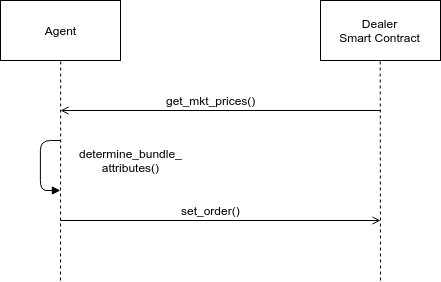
\includegraphics[width=.8\linewidth]{./figures/agent_bidding.png}
	\caption{Sequence of agent bidding}
	\label{figure:agent_bidding_figure}
\end{figure}

First, the agent gets the current market prices from the dealer's smart contract.
To obtain the market prices, the function \verb|getMktPrices()| of the dealer's smart contract is utilized.
The market prices are required for the determination of the preferred bundle set.

Next, the agent solves the bundle determination and initialize the class attributes
\verb|bundle_set| and \verb|bid|.
In turn, they are required for the next function call.
The corresponding implementation of this function is presented in Listing \ref{lst:determine_bundle}.

Finally, the agent sets the order in the dealer's smart contract.
To place the order in the contract, the function \verb|setOrder()| of the contract is utilized.
The implementation of the dealer's smart contract function is shown in the Listing \ref{lst:set_order_contract}.
Moreover, the implementation of the function \verb|set_order()| of the agent is 
also introduced in the Listing \ref{lst:set_order}.

\paragraph{Dealer's market clearing mechanism:}
To begin with, this activity refers to section \ref{sec:market_clearing_mechanism} and can be seen as
the technical implementation. Further, a sequence of all function 
calls for this activity is provided in Figure \ref{figure:dealers_mmp}.

First, the off-chain dealer gets the orders from the dealer's smart contract.
Therefore, the function \verb|get_orders()| of the agent (introduced in Listing \ref{lst:offchain_get_orders})
utilizes the function \verb|getOrder()| of the contract.

Then, the off-chain dealer creates and solves the MMP.
The implementation of both functions is outlined in appendix \ref{appendix:additional_offchain}.

\begin{figure}[htbp]
	\centering
	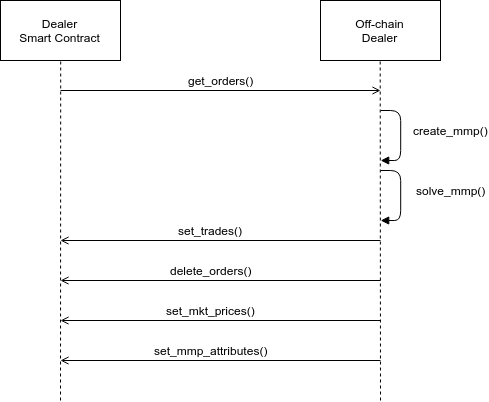
\includegraphics[width=.8\linewidth]{./figures/dealers_mmp.png}
	\caption{Sequence of dealer's market matching mechanism}
	\label{figure:dealers_mmp}
\end{figure}

After solving the MMP and the calculation of the respective 
trades, the off-chain dealer sets the trades in the dealer's smart contract.
Therefore, the function \verb|set_trade()| of the off-chain dealer (introduced in Listing \ref{lst:offchain_set_trades})
utilizes the function \verb|setTrade()| of the dealer's smart contract.

Afterwards, the off-chain dealer deletes the settled orders out of the dealer's
smart contract. 
To do this, the function \verb|delete_order()| of the off-chain dealer
utilizes the function \verb|deleteOrder()| of the dealer's smart contract.

In addition, the off-chain dealer sets the new market prices in the dealer's smart contract.
To set the new market prices, the function \verb|set_mkt_prices()| of the off-chain dealer 
utilizes the function \verb|setMktPrices()| of the dealer's smart contract.

Finally, the values of the MMP are set in the dealer's smart contract. 
They are used by the agents to verify the correctness of the calculated market prices.
Therefore, the function \verb|set_mmp_attributes()| of the off-chain dealer
utilizes the function \verb|setMMPAttributes()| of the dealer's smart contract.

\paragraph{Agent trade verification:}
To start, this activity covers the entire trade verification step of the agent. 
Likewise, a sequence of all function 
calls for this activity is provided in Figure \ref{figure:agents_trade_verification}.

\begin{figure}[htbp]
	\centering
	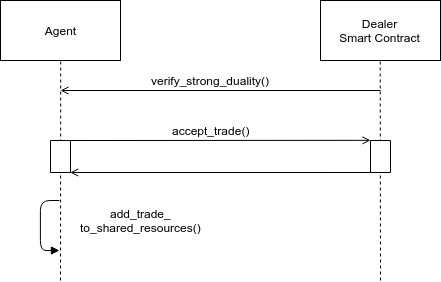
\includegraphics[width=.8\linewidth]{./figures/trade_verification.png}
	\caption{Sequence of agents trade verification}
	\label{figure:agents_trade_verification}
\end{figure}

First, the agent verifies if the conditions of the Strong Duality Theorem
are fulfilled.
Therefore, the function \verb|verify_strong_duality()| of the agent
(introduced in Listing \ref{lst:verify_trade})
utilizes the function \verb|getMMPAttributes()| of the dealer's smart contract.
As mentioned ealier in section \ref{sec:agent_bidding}, this function 
determine the class variable \verb|accept_trade| of type Boolean,
which indicates whether the trade is accepted or not.

Afer that, the agent informs the dealer's smart contract whether 
the trade is accepted or rejected.
For this, the function \verb|accept_trade()| of the agent
(introduced in Listing \ref{lst:accept_trade})
utilizes the function \verb|acceptTrade()| of the dealer's smart contract
(introduced in Listing \ref{lst:accept_trade_contract}).
In case of acceptance, the dealer's smart contract transfers the refunds 
to the agents and returns the respective bundle. Otherwise, in case of  
rejection, dealer's smart contract transfer the whole prepayment 
and deletes the respective trade.

Finally, the agent adds the trade to the shared resources. The invocation
of this function only affects if the trade was previously accepted. \newline

At the end of each iteration, the resource inventory of the dealer is recalculated.
Therefore the off-chain dealer calculates how much of the inventory is used for
the trades and settles this with the previous inventory.
Finally, the new calculated inventory is set in the dealer's smart contract.

\clearpage